\chapter{Esempi di modelli}


\begin{figure}[htbp]
    \centering
    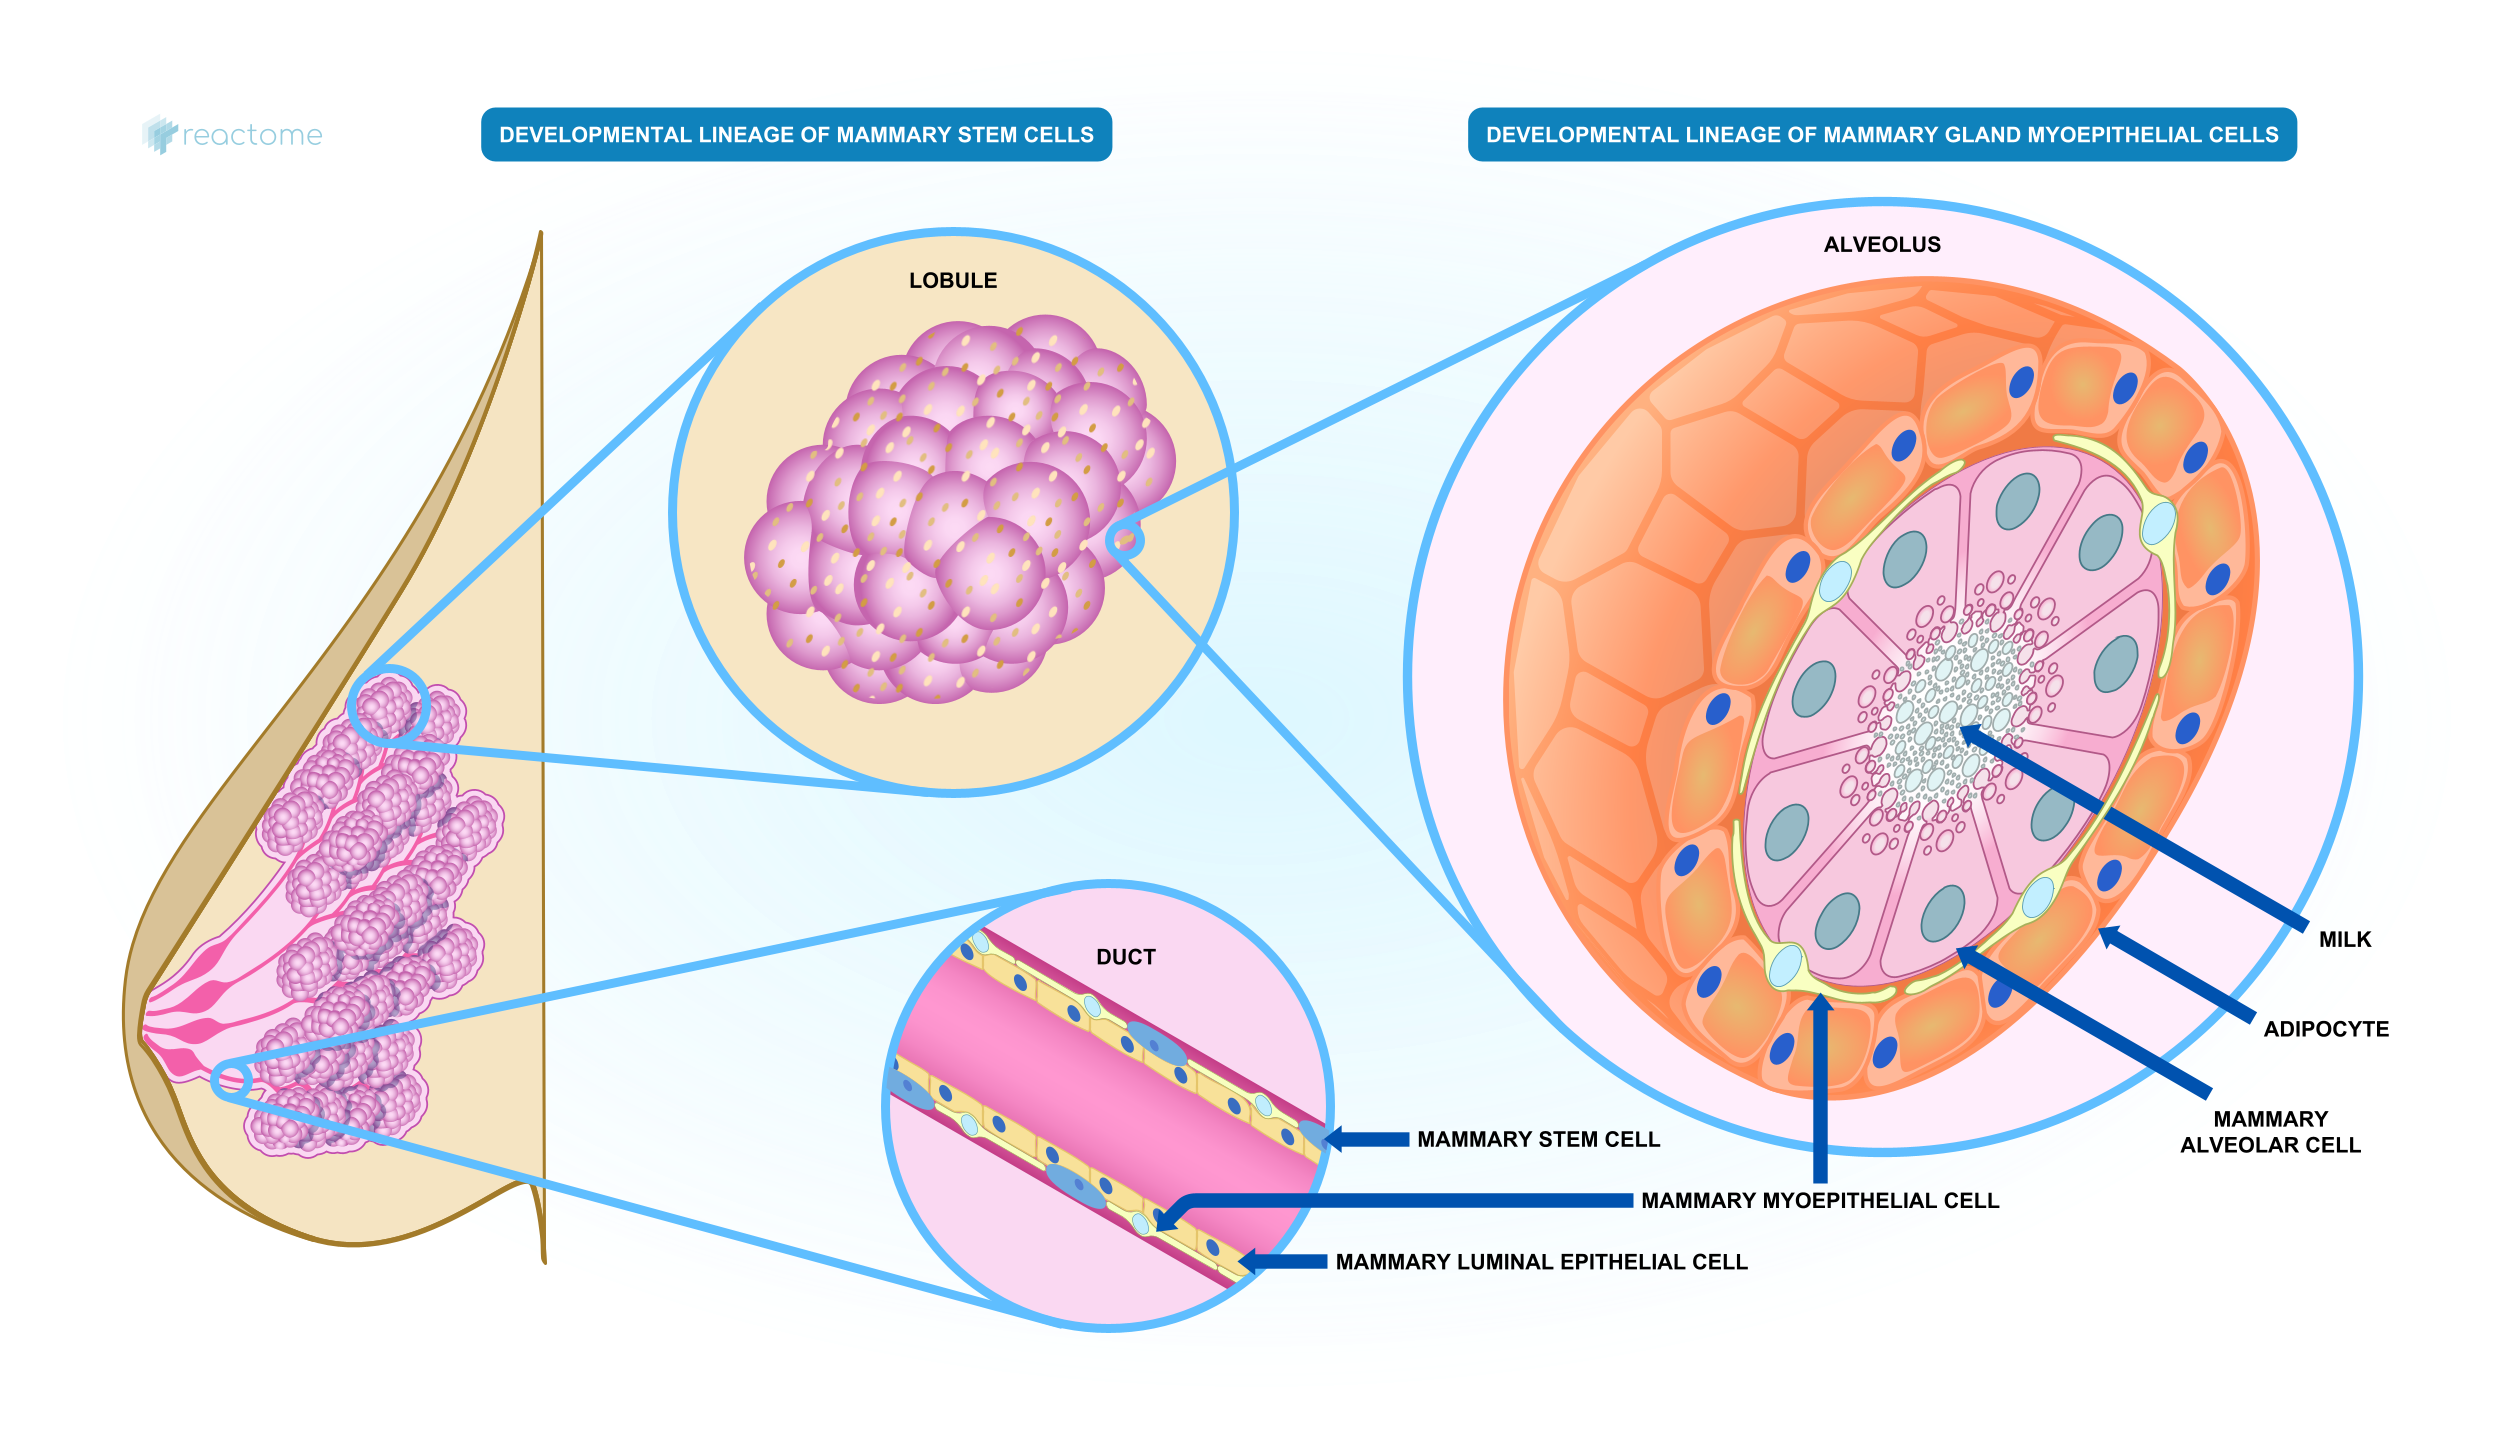
\includegraphics[width=\textwidth]{R-HSA-9938206.png}
    \caption{Rappresentazione del modello: R-HSA-9938206}
    \label{fig:R-HSA-9938206}
\end{figure}

Questo modello rappresenta lo sviluppo delle cellule staminali mammarie.

\begin{figure}[htbp]
    \centering
    \makebox[\textwidth][c]{%
        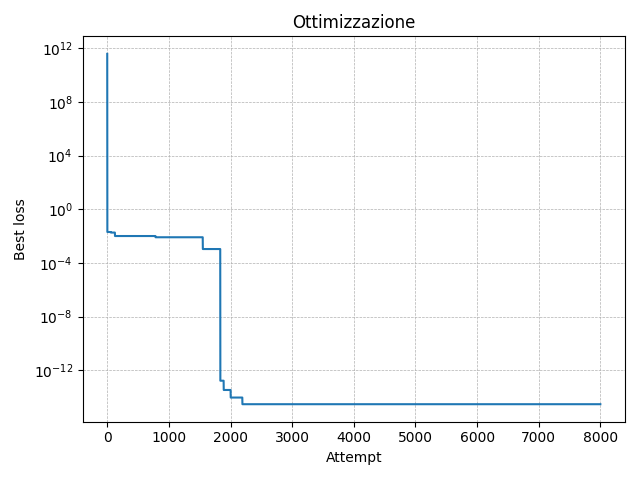
\includegraphics[width=0.5\textwidth]{plot_9938206.png}%
        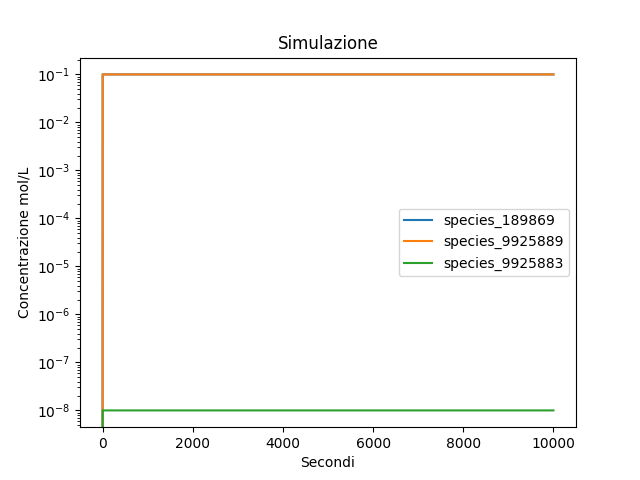
\includegraphics[width=0.5\textwidth]{simulation_9938206.png}%
    }%
    \caption{A sinistra c'è l'ottimizzazione fatta da Nevergrad dei parametri e a destra invece la simulazione.}
    \label{fig:due-immagini-affiancate}
\end{figure}

Il problema è stato vincolato in modo tale che le specie con id 189869 e 9925889 avessero come concentrazione media $0.1$ e che la specie 9925883 fosse la meno espressa.

Si possono vedere i risultati in \ref{fig:due-immagini-affiancate}

\begin{figure}[htbp]
    \centering
    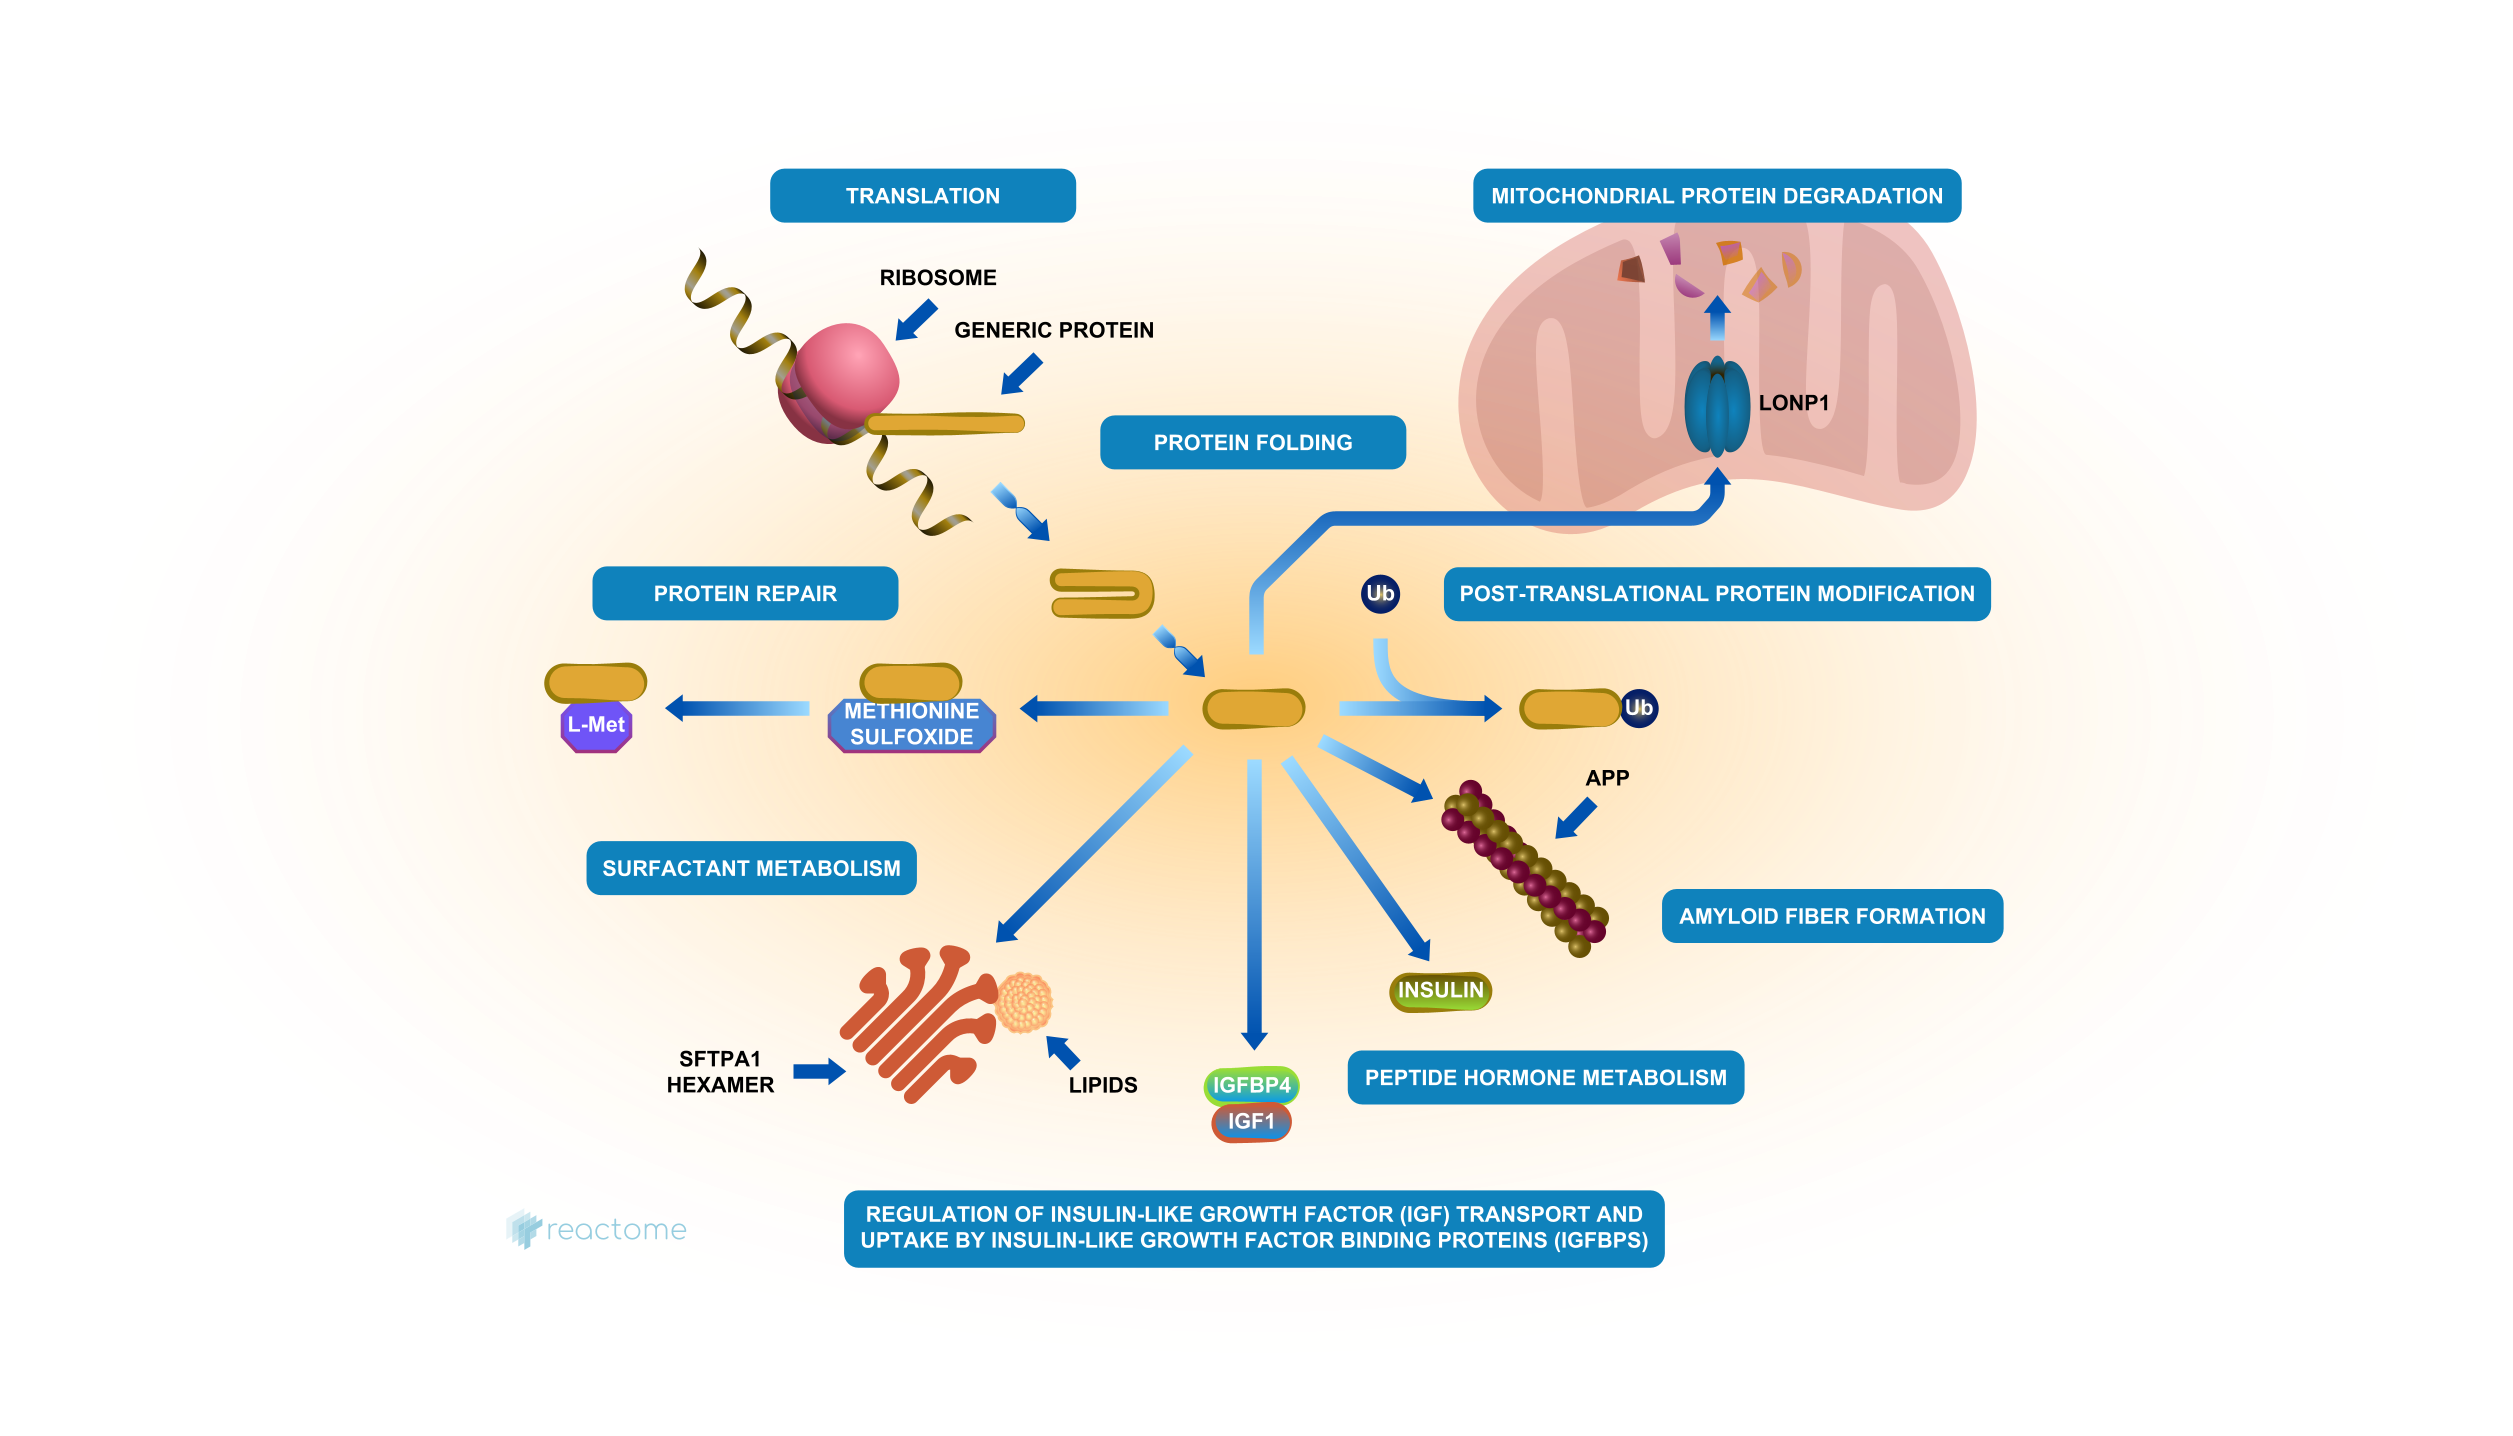
\includegraphics[width=\textwidth]{R-HSA-390471.png}
    \caption{Rappresentazione del modello: R-HSA-390471}
    \label{fig:R-HSA-390471}
\end{figure}

Per il modello \ref{fig:R-HSA-390471} è stata vincolata solo la stabilià e si possono vedere i risultati in \ref{fig:due-immagini-affiancate2}.

\begin{figure}[htbp]
    \centering
    \makebox[\textwidth][c]{%
        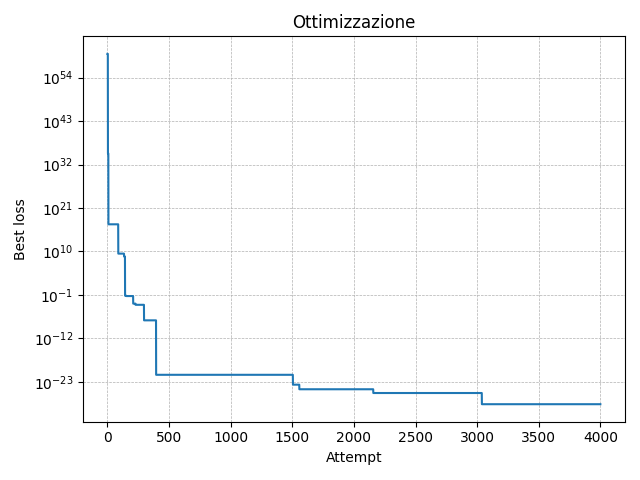
\includegraphics[width=0.5\textwidth]{plot_390471.png}%
        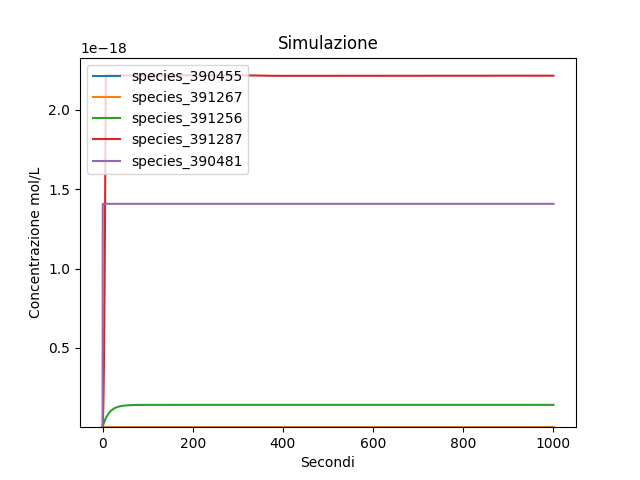
\includegraphics[width=0.5\textwidth]{simulation_390471.png}%
    }%
    \caption{A sinistra c'è l'ottimizzazione fatta da Nevergrad dei parametri e a destra invece la simulazione.}
    \label{fig:due-immagini-affiancate2}
\end{figure}